\documentclass[]{article}
\newcommand{\FileDepth}{../..}
\input{\FileDepth/Formats/AssignmentBasics.tex}
%opening
\newcommand{\SecType}{X}
\newcommand{\Week}{X}
\title{Vectors in a Garden}
\author{Benjamin Bauml}
\date{Summer 2024}
\pagestyle{fancy}
\rhead{PH 211}
\chead{Summer 2024}
\lhead{Week \Week}

% For Assignment, leave Purpose as 1. For Worksheet, set to 2. For Student Solution, set to 3. For Teacher Solution, set to 4.
% If you want keep the pieces from being called manually, set DefOnly to 0.
\newcommand{\Purpose}{4}
\newcommand{\DefOnly}{1}

\input{\FileDepth/Formats/Assignment20240519.tex}

%\newcommand{\FBDaxes}[4][2]{
	\begin{scope}[shift={(#2)},rotate=#3]
		% x-axis
		\draw[thick,->] (-#1,0) -- (#1,0);
		\node[anchor=west] at (#1,0) {$x$};
		% y-axis
		\draw[thick,->] (0,-#1) -- (0,#1);
		\node[anchor=south] at (0,#1) {$y$};
		\coordinate (#4) at (0,0);
	\end{scope}
}
\newcommand{\FBDvectorMA}[4]{
	\begin{scope}[shift={(#1)}]
		\coordinate (#4tip) at ({#2*cos(#3)},{#2*sin(#3)});
		\draw[ultra thick,blue,->] (#1) -- (#4tip);
	\end{scope}
}
\newcommand{\FBDvectorXY}[3]{
	\begin{scope}[shift={(#1)}]
		\coordinate (#3tip) at (#2);
		\draw[ultra thick,blue,->] (0,0) -- (#3tip);
	\end{scope}
}
\newcommand{\FBDdot}[1]{
	\filldraw[black] (#1) circle (3pt);
}
\newcommand{\FBDbox}[5][1]{
	\begin{scope}[shift={(#2)},rotate=#3]
		\filldraw[color=black,fill=white,thick] ({-#1/2},{#1/2}) -- ({-#1/2},{-#1/2}) -- ({#1/2},{-#1/2}) -- ({#1/2},{#1/2}) -- cycle;
		% Left side coordinates
		\coordinate (#4ltq) at ({-#1/2},{#1/4});
		\coordinate (#4lcent) at ({-#1/2},0);
		\coordinate (#4lbq) at ({-#1/2},{-#1/4});
		% right side coordinates
		\coordinate (#4rtq) at ({#1/2},{#1/4});
		\coordinate (#4rcent) at ({#1/2},0);
		\coordinate (#4rbq) at ({#1/2},{-#1/4});
		% top coordinates
		\coordinate (#4tlq) at ({-#1/4},{#1/2});
		\coordinate (#4tcent) at (0,{#1/2});
		\coordinate (#4trq) at ({#1/4},{#1/2});
		% bottom coordinates
		\coordinate (#4blq) at ({-#1/4},{-#1/2});
		\coordinate (#4bcent) at (0,{-#1/2});
		\coordinate (#4brq) at ({#1/4},{-#1/2});
		% corners
		\coordinate (#4tl) at ({-#1/2},{#1/2});
		\coordinate (#4tr) at ({#1/2},{#1/2});
		\coordinate (#4bl) at ({-#1/2},{-#1/2});
		\coordinate (#4br) at ({#1/2},{-#1/2});
		\node at (0,0) {#5};
	\end{scope}
}
%\newcommand{\MVec}[3][0]{%Creates a momentum vector of length #3 centered at #2 and rotated #1 degrees counterclockwise.
	\begin{scope}[rotate=#1,shift={(#2)}]
		\draw[->,thick] ({-#3/2},0) -- ({#3/2},0);
	\end{scope}
}
\newcommand{\MDot}[1]{%Creates a dot at #1 to represent a zero vector.
	\filldraw (#1) circle (1pt);
}
\newcommand{\MVDRows}[2][4.5]{%Creates the rows (initial, delta, final) of a momentum vector diagram. The optional argument determines the width of the table, and defaults to a good length for three columns (two objects and the total system). The non-optional argument gives a coordinate name (not displayed) to the diagram.
	\begin{scope}
		%\draw[thick] (0,5.5) -- (0,0);
		\draw[thick] (-1,4.5) -- (#1,4.5);
		\node at (-0.5,3.75) {$\vec{p}_{i}$};
		\draw[thick] (-1,3) -- (#1,3);
		\node at (-0.5,2.25) {$\Delta\vec{p}$};
		\draw[thick] (-1,1.5) -- (#1,1.5);
		\node at (-0.5,0.75) {$\vec{p}_{f}$};
		\coordinate (#2) at (0,5);
	\end{scope}
}
\newcommand{\MVDCol}[4][0.75]{%Creates a column for an object in a momentum vector diagram. The first (non-optional) argument is the coordinate name (not displayed) of the column, while the second is the displayed column header. The first argument also names the three entries down the column. The third argument anchors the column, so it should either be the coordinate name of the MVD (for the first column) or the coordinate name of the previous column. The optional argument indicates how far the center of the column should be from the previous column's edge, and defaults to 0.75.
	\begin{scope}[shift={(#4)}]
		\node at (#1,0) {#3};
		%\draw[thick] ({#1*2},0.5) -- ({#1*2},-5);
		\draw[thick] (0,0.5) -- (0,-5);
		\coordinate (#2init) at (#1,-1.25);
		\coordinate (#2delt) at (#1,-2.75);
		\coordinate (#2fin) at (#1,-4.25);
		\coordinate (#2) at ({#1*2},0);
	\end{scope}
}

\begin{document}
\maketitle

\Problem{Vectors in a Garden}{\GardenVec}{
You visit a garden with a trail that includes the following landmarks.
\begin{itemize}
	\item Red roses at $\vec{r}_{r} = -3a\hat{x}$
	\item White roses at $\vec{r}_{w} = +4a\hat{x}$
	\item A pond at $\vec{r}_{p}=0\hat{x}$
	\item A bench at $\vec{r}_{b}=-a\hat{y}$
	\item A bridge over a creek at $\vec{r}_{c}=-a\hat{x}$
	\item A statue at $\vec{r}_{s}=+2a\hat{x}$
\end{itemize}
}
\ProblemSub{\GardenVecI}{
(1) Sketch and label the garden and its landmarks.
}
\Solution{\GardenVecISol}{

\begin{figure}[h]
	\centering
	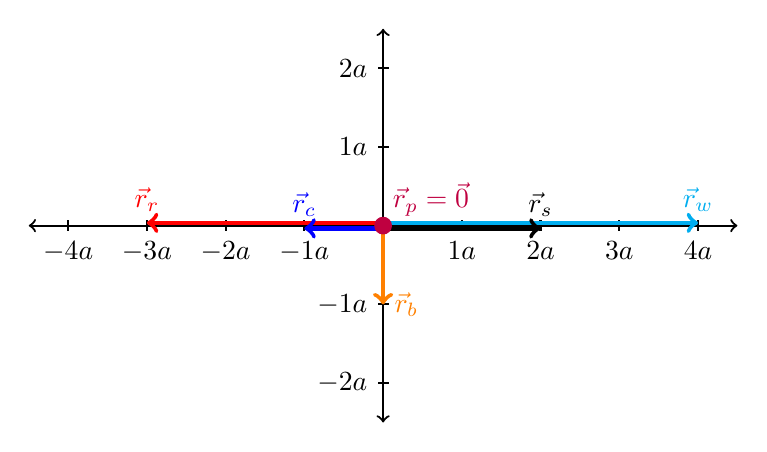
\begin{tikzpicture}
		\draw[thick,<->] (-4.5,0) -- (4.5,0);
		\foreach \x in {-4,-3,-2,-1,1,2,3,4}
			\draw[thick] (\x,2pt) -- (\x,-2pt) node[anchor=north] {$\x a$};
		\draw[thick,<->] (0,-2.5) -- (0,2.5);
		\foreach \y in {-2,-1,1,2}
			\draw[thick] (2pt,\y) -- (-2pt,\y) node[anchor=east] {$\y a$};
		\draw[ultra thick,red,->,shift={(0,1pt)}] (0,0) -- (-3,0) node[anchor=south] {$\vec{r}_{r}$};
		\draw[ultra thick,blue,->,shift={(0,-1pt)}] (0,0) -- (-1,0) node[anchor=south] {$\vec{r}_{c}$};
		\draw[ultra thick,cyan,->,shift={(0,1pt)}] (0,0) -- (4,0) node[anchor=south] {$\vec{r}_{w}$};
		\draw[ultra thick,black,->,shift={(0,-1pt)}] (0,0) -- (2,0) node[anchor=south] {$\vec{r}_{s}$};
		\draw[ultra thick,orange,->] (0,0) -- (0,-1) node[anchor=west] {$\vec{r}_{b}$};
		\filldraw[purple] (0,0) circle (3pt) node[anchor=south west] {$\vec{r}_{p}=\vec{0}$};
	\end{tikzpicture}
\end{figure}
}
\ProblemSub{\GardenVecII}{
(2) Find the following displacement vectors using both symbols and diagrams.
}
\Solution{\GardenVecIISol}{

A displacement vector, $\Delta \vec{r}$, can be thought of as the difference of the final position vector, $\vec{r}_{f}$, and the initial position vector, $\vec{r}_{i}$:
\[
\Delta\vec{r} = \vec{r}_{f}-\vec{r}_{i}.
\]
It can also be thought of as the vector that, when added to $\vec{r}_{i}$, gives you $\vec{r}_{f}$:
\[
\Delta\vec{r} = \vec{r}_{f}-\vec{r}_{i}.
\]
As such, $\Delta\vec{r}$ points from the tip of $\vec{r}_{i}$ to the tip of $\vec{r}_{f}$:
\begin{figure}[h]
	\centering
	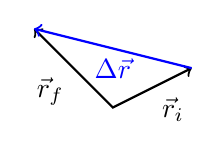
\begin{tikzpicture}
		\draw[thick,<->] (-1,1) -- (0,0) -- (1,0.5);
		\node[anchor=north east] at (-0.5,0.5) {$\vec{r}_{f}$};
		\node[anchor=north west] at (0.5,0.25) {$\vec{r}_{i}$};
		\draw[thick,blue,->] (1,0.5) -- (-1,1);
		\node[anchor=north,blue] at (0,0.75) {$\Delta\vec{r}$};
	\end{tikzpicture}
\end{figure}
}
\ProblemSub{\GardenVecIIA}{
(a) From the red roses to the white roses
}
\Solution{\GardenVecIIASol}{

\begin{figure}[h]
	\centering
	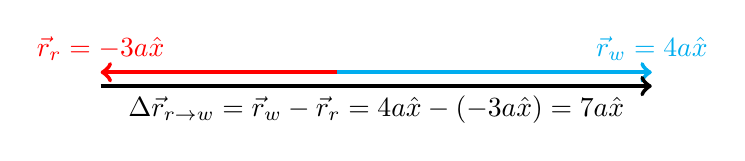
\begin{tikzpicture}
		\draw[ultra thick,red,->] (0,0) -- (-3,0) node[anchor=south] {$\vec{r}_{r}=-3a\hat{x}$};
		\draw[ultra thick,cyan,->] (0,0) -- (4,0) node[anchor=south] {$\vec{r}_{w}=4a\hat{x}$};
		\draw[ultra thick,black,->,shift={(0,-5pt)}] (-3,0) -- (4,0);
		\node[anchor=north] at (0.5,-5pt) {$\Delta\vec{r}_{r\to w} = \vec{r}_{w}-\vec{r}_{r} = 4a\hat{x} - (-3a\hat{x}) = 7a\hat{x}$};
	\end{tikzpicture}
\end{figure}
}
\ProblemSub{\GardenVecIIB}{
(b) From the pond to the red roses
}
\Solution{\GardenVecIIBSol}{

\begin{figure}[h]
	\centering
	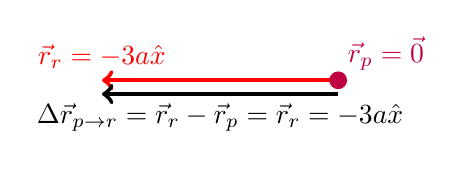
\begin{tikzpicture}
		\draw[ultra thick,red,->] (0,0) -- (-3,0) node[anchor=south] {$\vec{r}_{r}=-3a\hat{x}$};
		\filldraw[purple] (0,0) circle (3pt) node[anchor=south west] {$\vec{r}_{p}=\vec{0}$};
		\draw[ultra thick,black,->,shift={(0,-5pt)}] (0,0) -- (-3,0);
		\node[anchor=north] at (-1.5,-5pt) {$\Delta\vec{r}_{p\to r} = \vec{r}_{r}-\vec{r}_{p} = \vec{r}_{r} = -3a\hat{x}$};
	\end{tikzpicture}
\end{figure}
}
\ProblemSub{\GardenVecIIC}{
(c) From the bench to the statue
}
\Solution{\GardenVecIICSol}{

\begin{figure}[h]
	\centering
	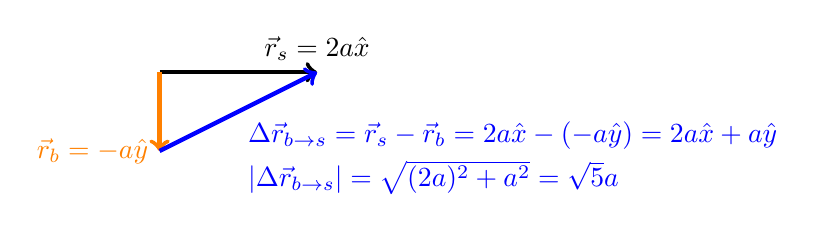
\begin{tikzpicture}
		\draw[ultra thick,black,->] (0,0) -- (2,0) node[anchor=south] {$\vec{r}_{s}=2a\hat{x}$};
		\draw[ultra thick,orange,->] (0,0) -- (0,-1) node[anchor=east] {$\vec{r}_{b}=-a\hat{y}$};
		\draw[ultra thick,blue,->] (0,-1) -- (2,0);
		\node[anchor=north west,blue] at (1,-0.5) {$\Delta\vec{r}_{b\to s} = \vec{r}_{s}-\vec{r}_{b} = 2a\hat{x} - (-a\hat{y}) = 2a\hat{x} + a\hat{y}$};
		\node[anchor=north west,blue] at (1,-1) {$\left|\Delta\vec{r}_{b\to s}\right| = \sqrt{(2a)^{2}+a^{2}} = \sqrt{5}a$};
	\end{tikzpicture}
\end{figure}
}
\end{document}